\section{任务三}
任务三要求在从 4 个转子中选择 3 个后进行加密。为便于说明，先给出三个转子固定、但转子顺序未知时的密钥空间。

三个固定转子的排列有 $3!$ 种，每个转子的起始位置有 26 种可能，因此

\begin{equation*}
    N_{K_2}=3!\times26^3=105,456\approx2^{16.69}.
\end{equation*}

按照实验指导书和参考程序中的限制，接线板最多有 6 条接线。严格计算所有允许的接线数量时，

\begin{equation*}
    N_{K_1}=\sum_{l=0}^{6}\frac{26!}{(26-2l)!2^l l!}
    =105,578,918,576\approx2^{36.62}.
\end{equation*}

因此，三个转子固定但顺序未知时的完整密钥空间为

\begin{equation*}
    N=N_{K_1}N_{K_2}
    =11,133,930,437,350,656
    \approx2^{53.31}.
\end{equation*}

若按照最大接线数 $l=6$ 的最大项进行数量级估计，则 $N_{K_1}(6)\approx2^{36.55}$，相应的总密钥空间约为 $2^{53.23}$，同样可以近似记为 $2^{53}$。

当从 4 个转子中选择 3 个并安排顺序时，转子部分的排列数量变为

\begin{equation*}
    N_{K_2}'=P_4^3\times26^3
    =24\times26^3
    =421,824\approx2^{18.69}.
\end{equation*}

接线板的可能数量不变，因此任务三的完整密钥空间为

\begin{equation*}
    N'=N_{K_1}N_{K_2}'
    =44,535,721,749,402,624
    \approx2^{55.31}.
\end{equation*}

若采用 $l=6$ 最大项估算，则

\begin{equation*}
    N'_{l=6}=N_{K_1}(6)N_{K_2}'
    =42,347,667,057,696,000
    \approx2^{55.23}.
\end{equation*}

因此任务三理论上需要猜测约 $2^{55}$ 个完整密钥。

对任务一中的 Enigma 加密程序进行性能测试，采用 1000 条长度为 6 的随机明文并统计加密时间，测试结果如下：
\begin{figure}[H]
    \centering
    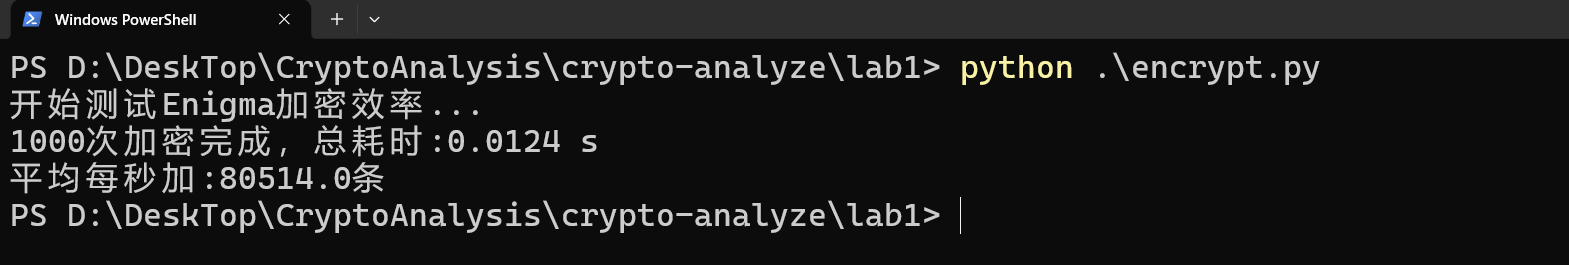
\includegraphics[width = 1\textwidth]{figures/task3_encrypt_efficiency.png}
    \caption{测试Enigma加密效率}
\end{figure}
测试结果显示每秒约可完成 80514 次加密\footnote{测试明文长度均为 6，随机明文在计时前生成；测试循环中复用同一台 Enigma 机器，因此测量的是连续加密吞吐量。}。若采用严格的“不超过 6 条接线”密钥空间进行估计，则直接穷举所需时间为

\begin{equation*}
    T=\frac{N'}{80514}
    \approx5.53\times10^{11}\text{ s}
    \approx9.22\times10^9\text{ min}
    \approx6.40\times10^6\text{ d}
    \approx1.75\times10^4\text{ 年}.
\end{equation*}

若按 $l=6$ 最大项近似，则所需时间约为 $5.26\times10^{11}$ s，即约 $1.67\times10^4$ 年。两种计算结果均表明，在个人计算机上直接穷举任务三的完整密钥空间完全不可行。
